\section{Final Results (mode shapes visualization)}
\label{sec:final_results_B}

In this section, the identified mode shapes identified from the experimental data are reported.

\begin{figure}[H]
    \centering
    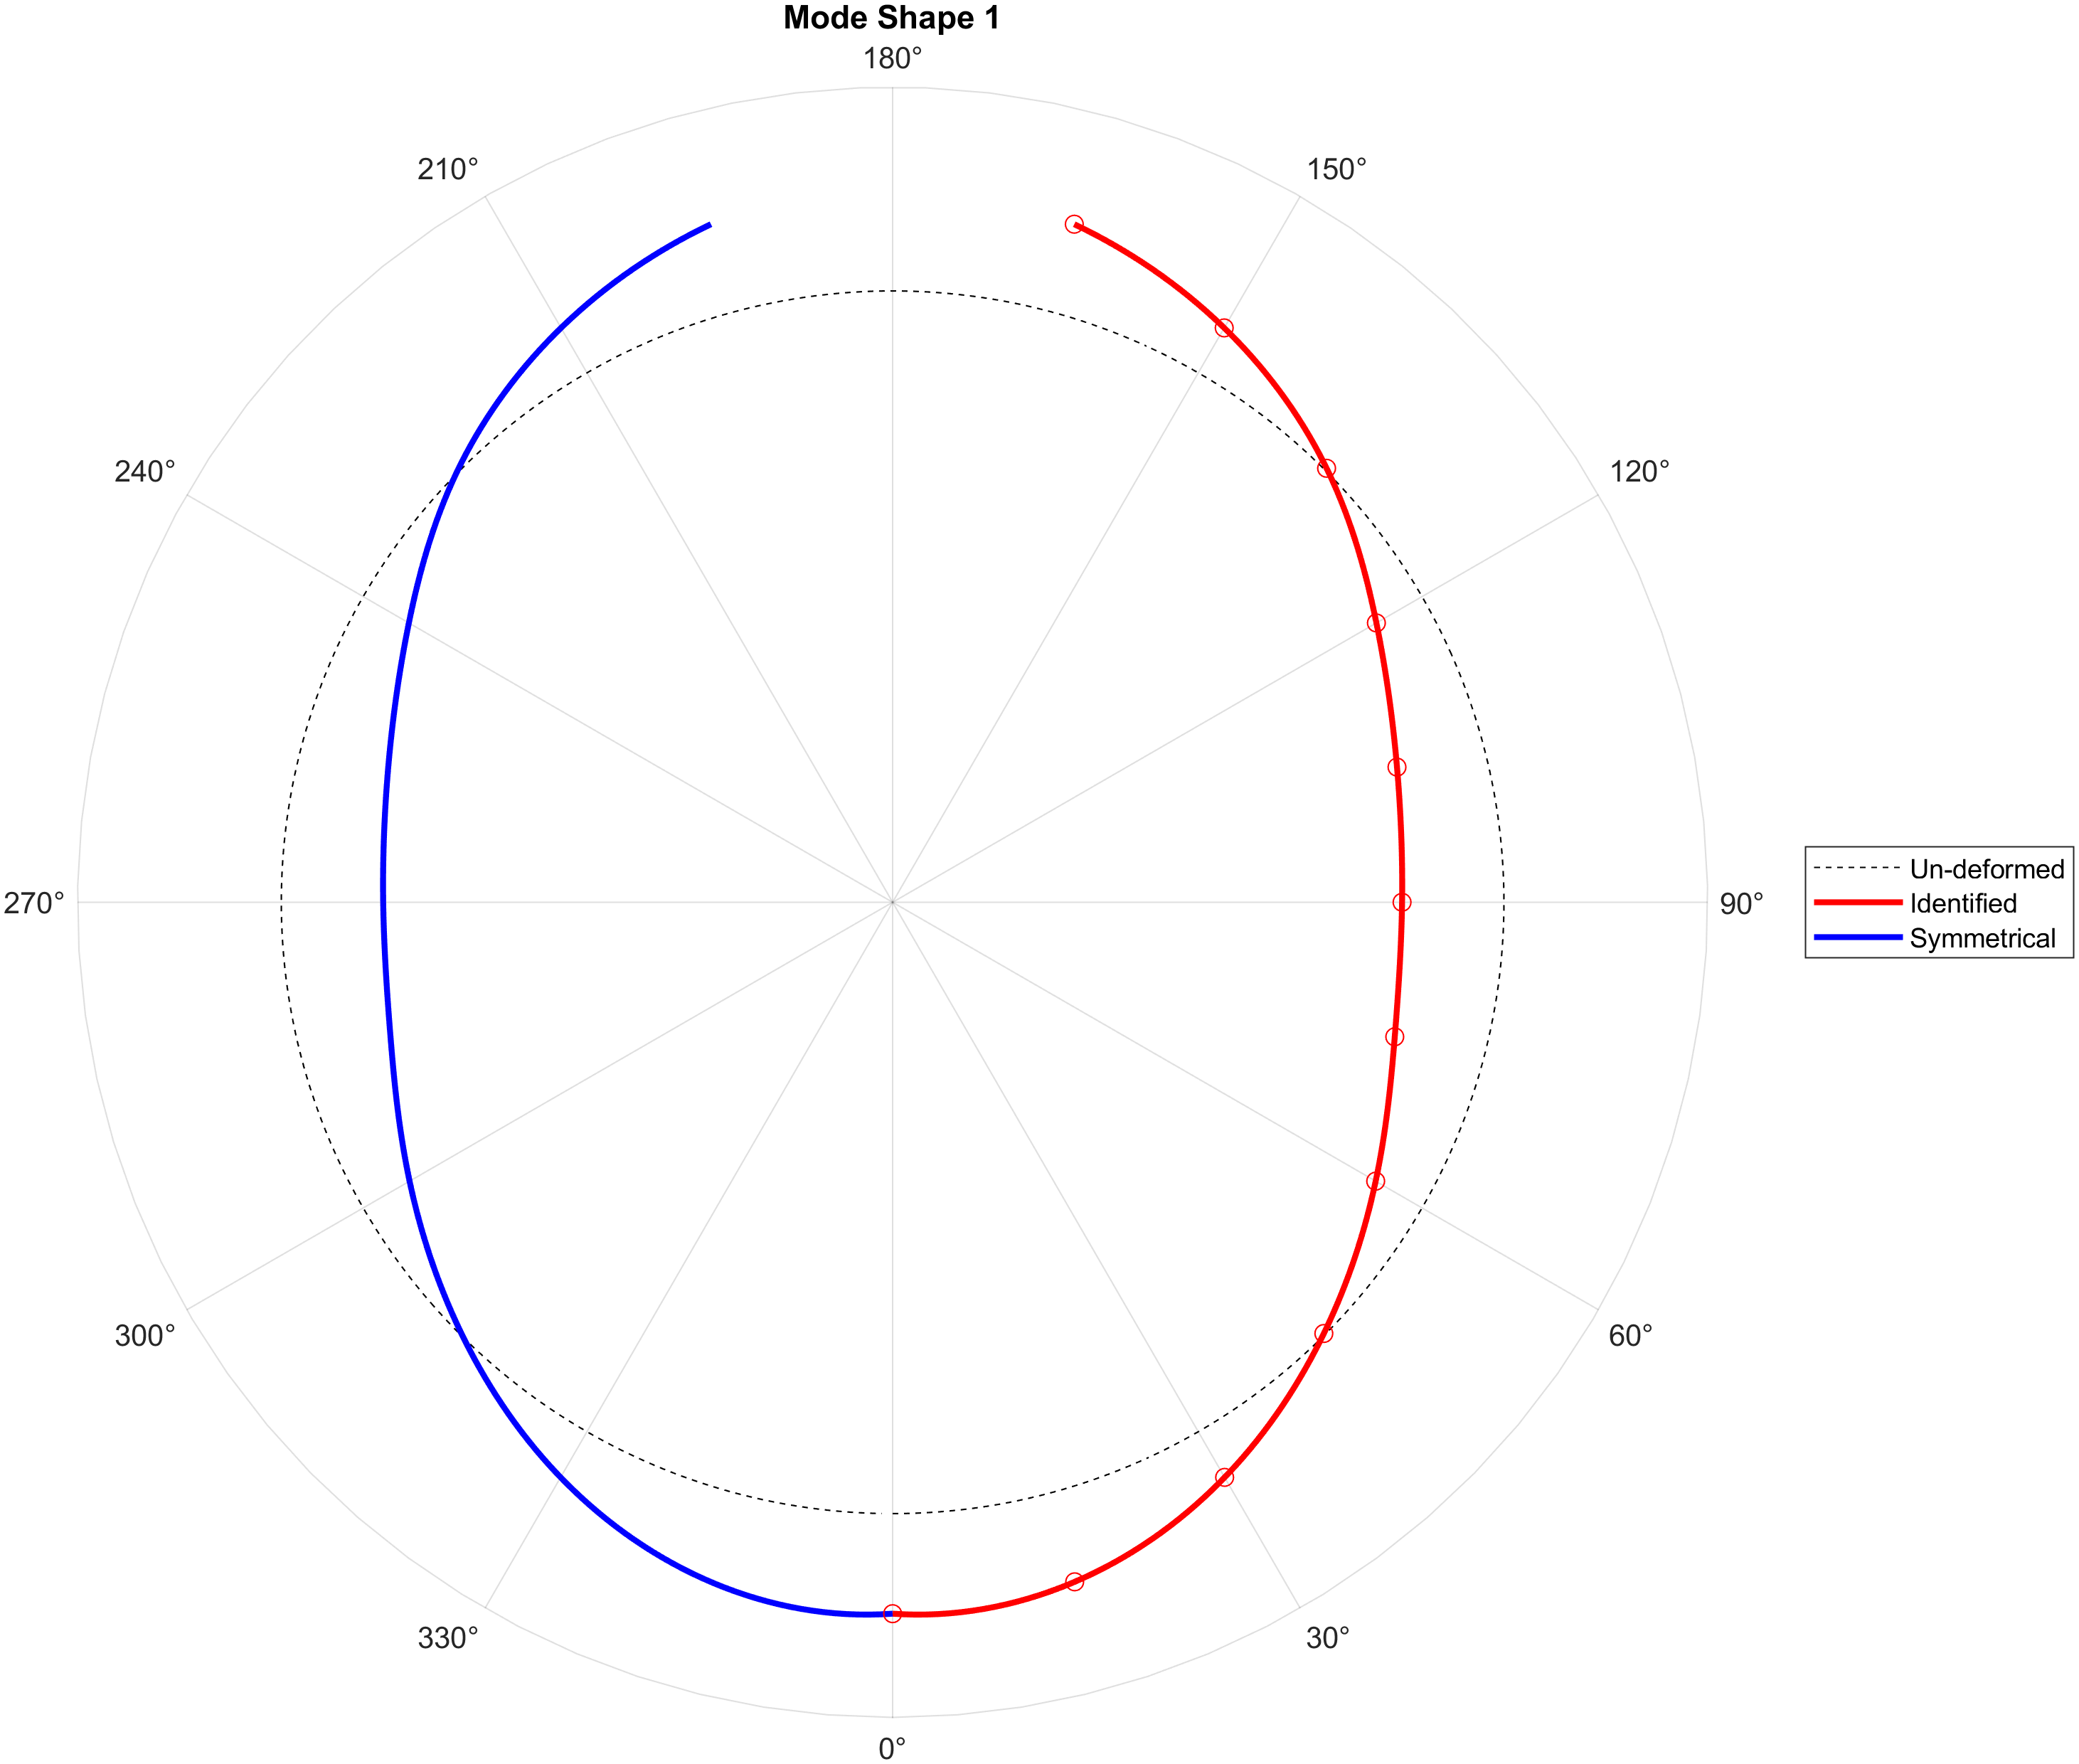
\includegraphics[width=0.45\textwidth]{img/MATLAB/Part_B/ModeShape_01.png}
    \hfill
    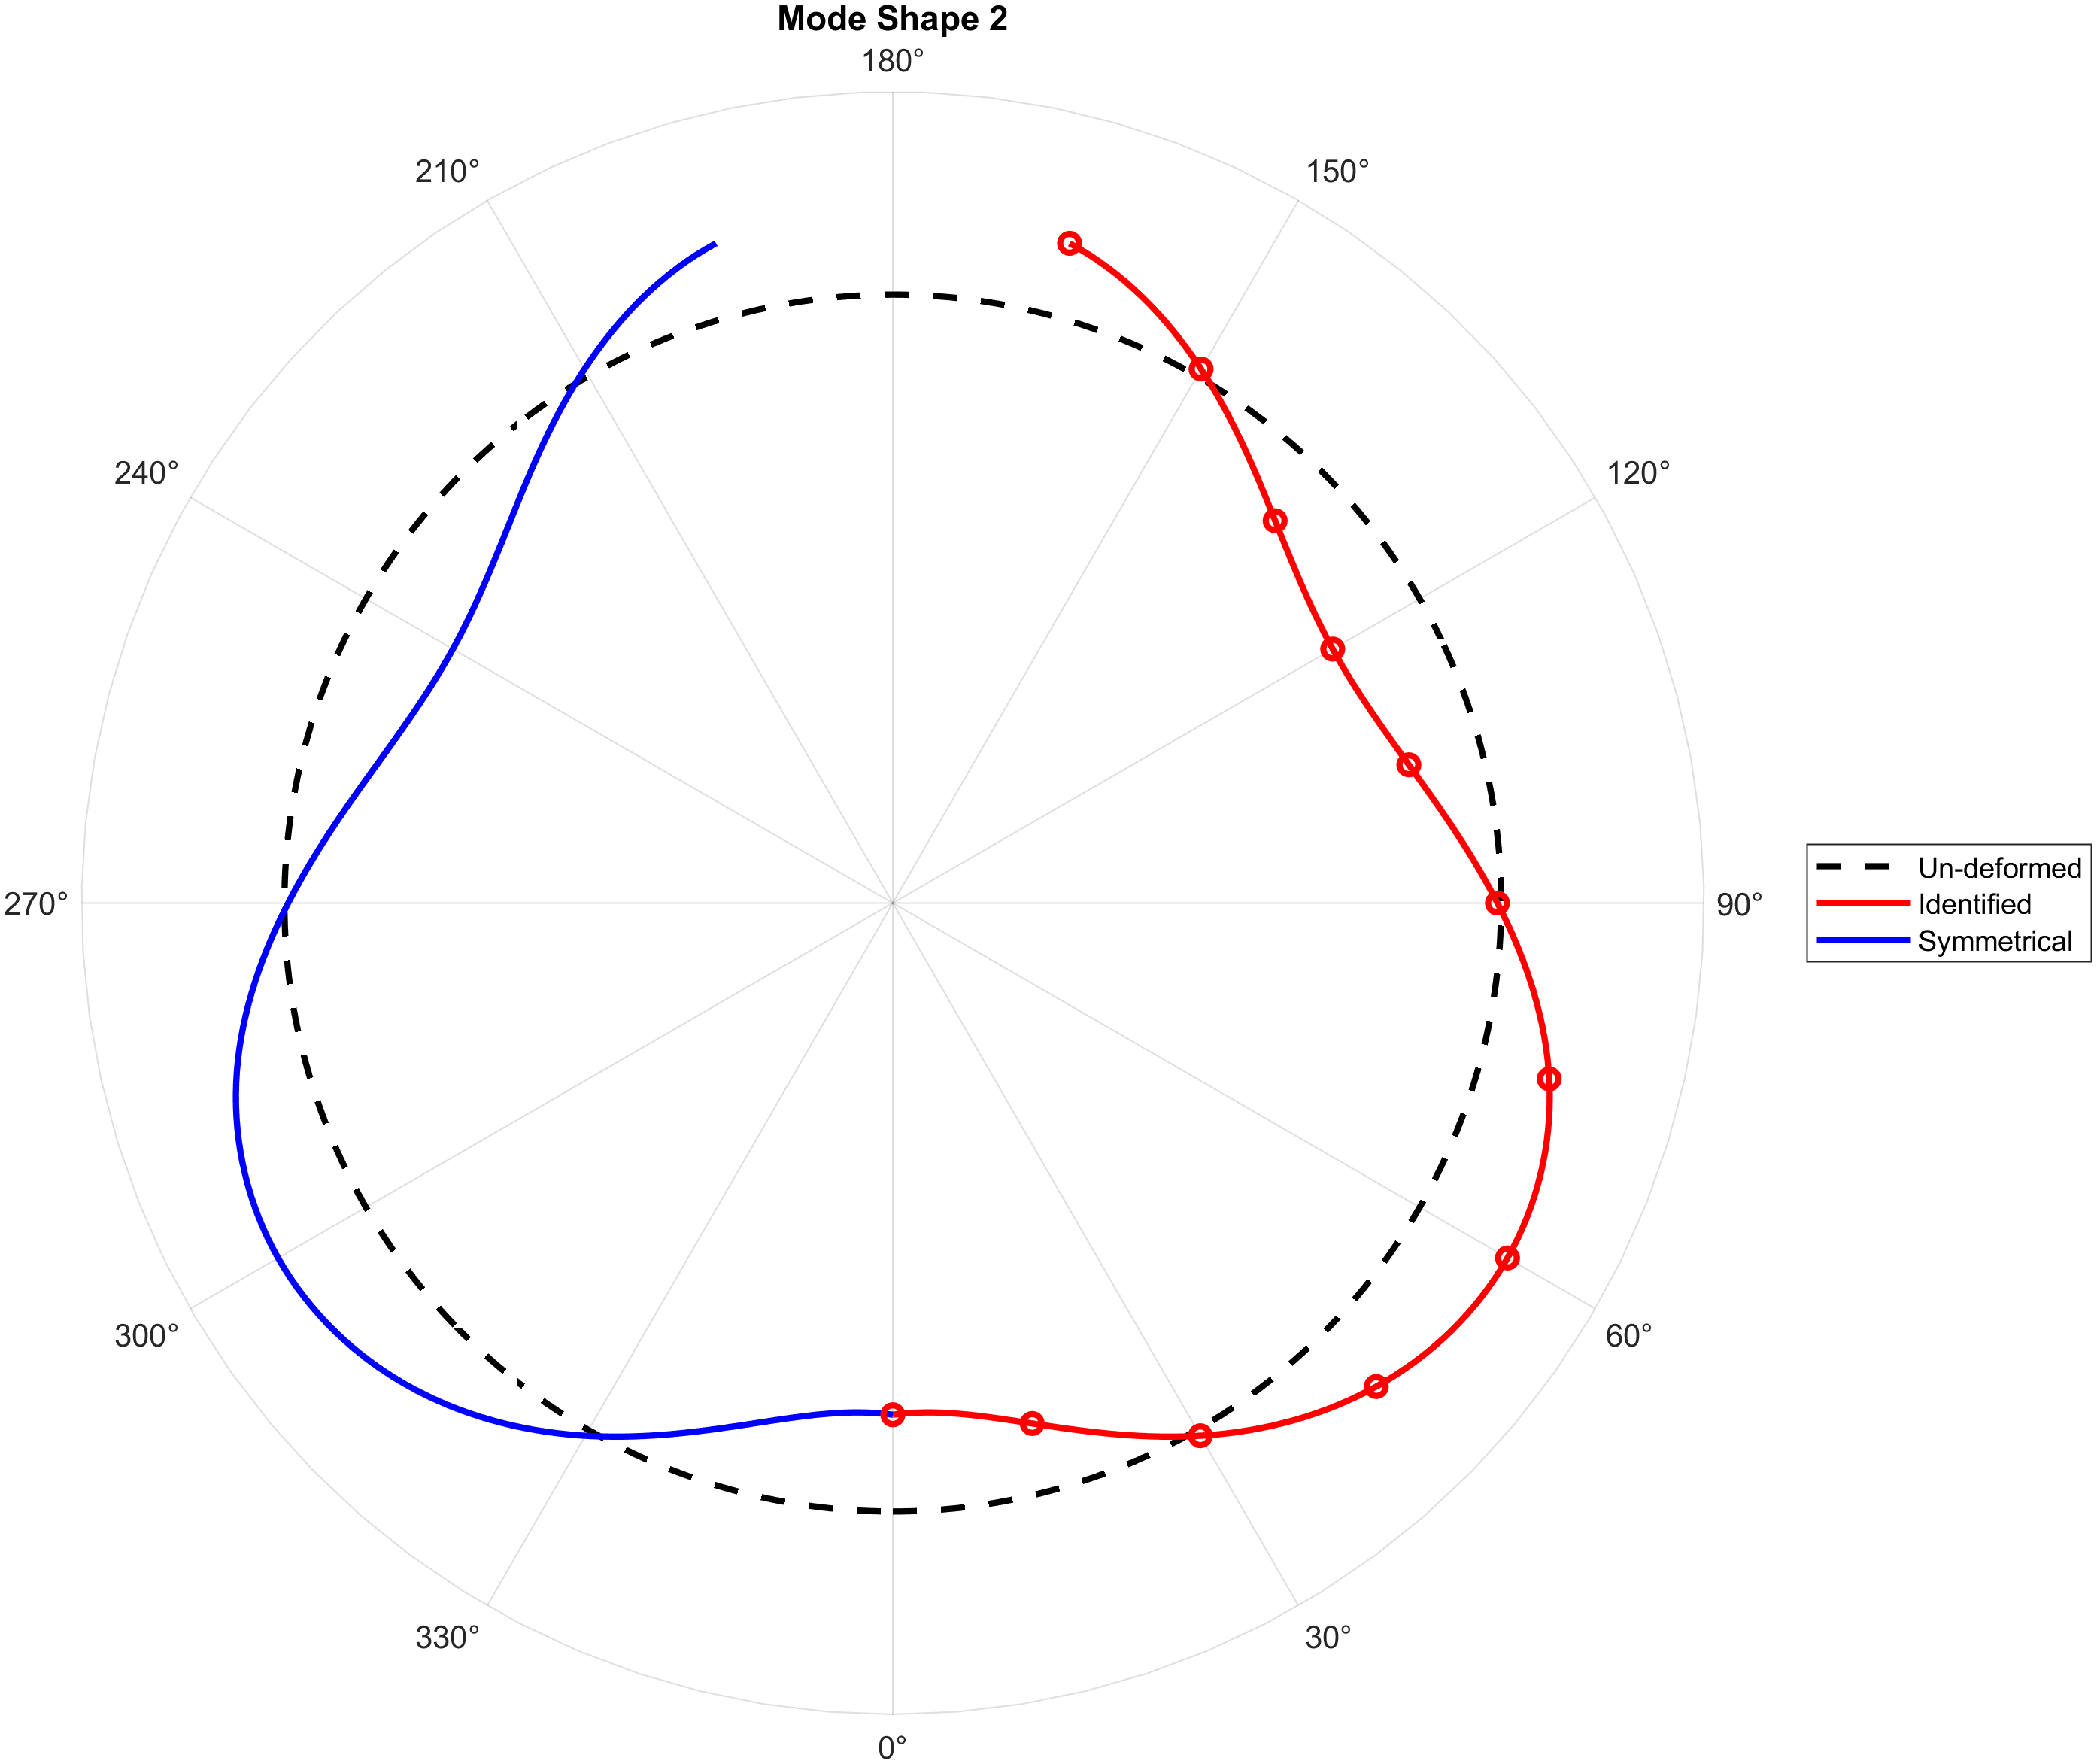
\includegraphics[width=0.45\textwidth]{img/MATLAB/Part_B/ModeShape_02.png}
    \caption{Identified (numerically) first two mode shapes of the system.}
    \label{fig:mode_shapes}
\end{figure}

Notice that those graph must be interpreted as axial displacements with respect to the un-deformed system.
Basically, the more the colored line are far from the black dashed line, the more the system is axially deformed in that region.
Moreover, the position of the colored lines with respect to the black dashed line (external or internal) indicates the direction of the deformation with respect to the un-deformed plane of the system.

The first mode shape (Figure \ref{fig:mode_shapes}, left) can also be visualized in a 3D way that to a FEA simulation performed in \cite{FEM_rail_wheel}.

\begin{figure}[H]
    \centering
    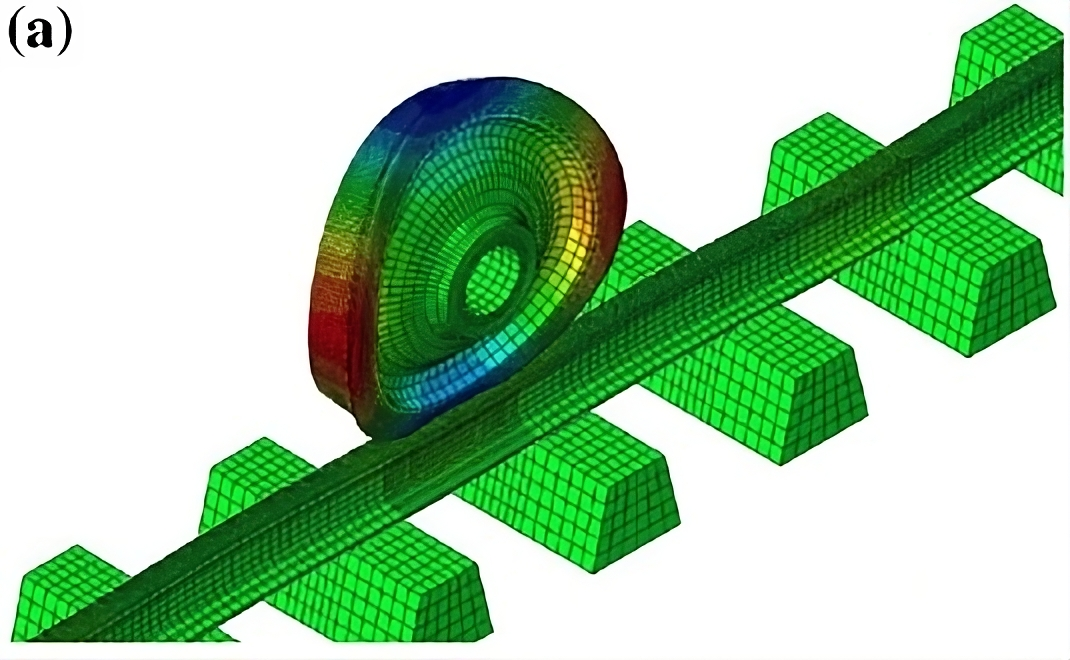
\includegraphics[width=0.7\textwidth]{img/wheel-FEM-first-mode-shape.png}
    \caption{First mode shape of the system visualized in a 3D way. Credit to \cite{FEM_rail_wheel}.}
    \label{fig:mode_shape_3D}
\end{figure}

As a final remark, we report in Table \ref{tab:mode_shapes_parameters} the identified parameters for the first two mode shapes of the system.

\begin{table}[H]
    \centering
    \begin{tabular}{lcc}
        \hline
        Mode & Frequency [Hz] & Damping ratio [\%] \\
        \hline
        1    & 667.324        & 0.75 \%            \\
        2    & 1625.312       & 0.59 \%            \\
        \hline
    \end{tabular}
    \caption{Identified parameters for the first two mode shapes of the system.}
    \label{tab:mode_shapes_parameters}
\end{table}

